\section{CHAPTER 6: GENERATOR \cite{j420}}
\begin{figure}[h!]
    \centering
    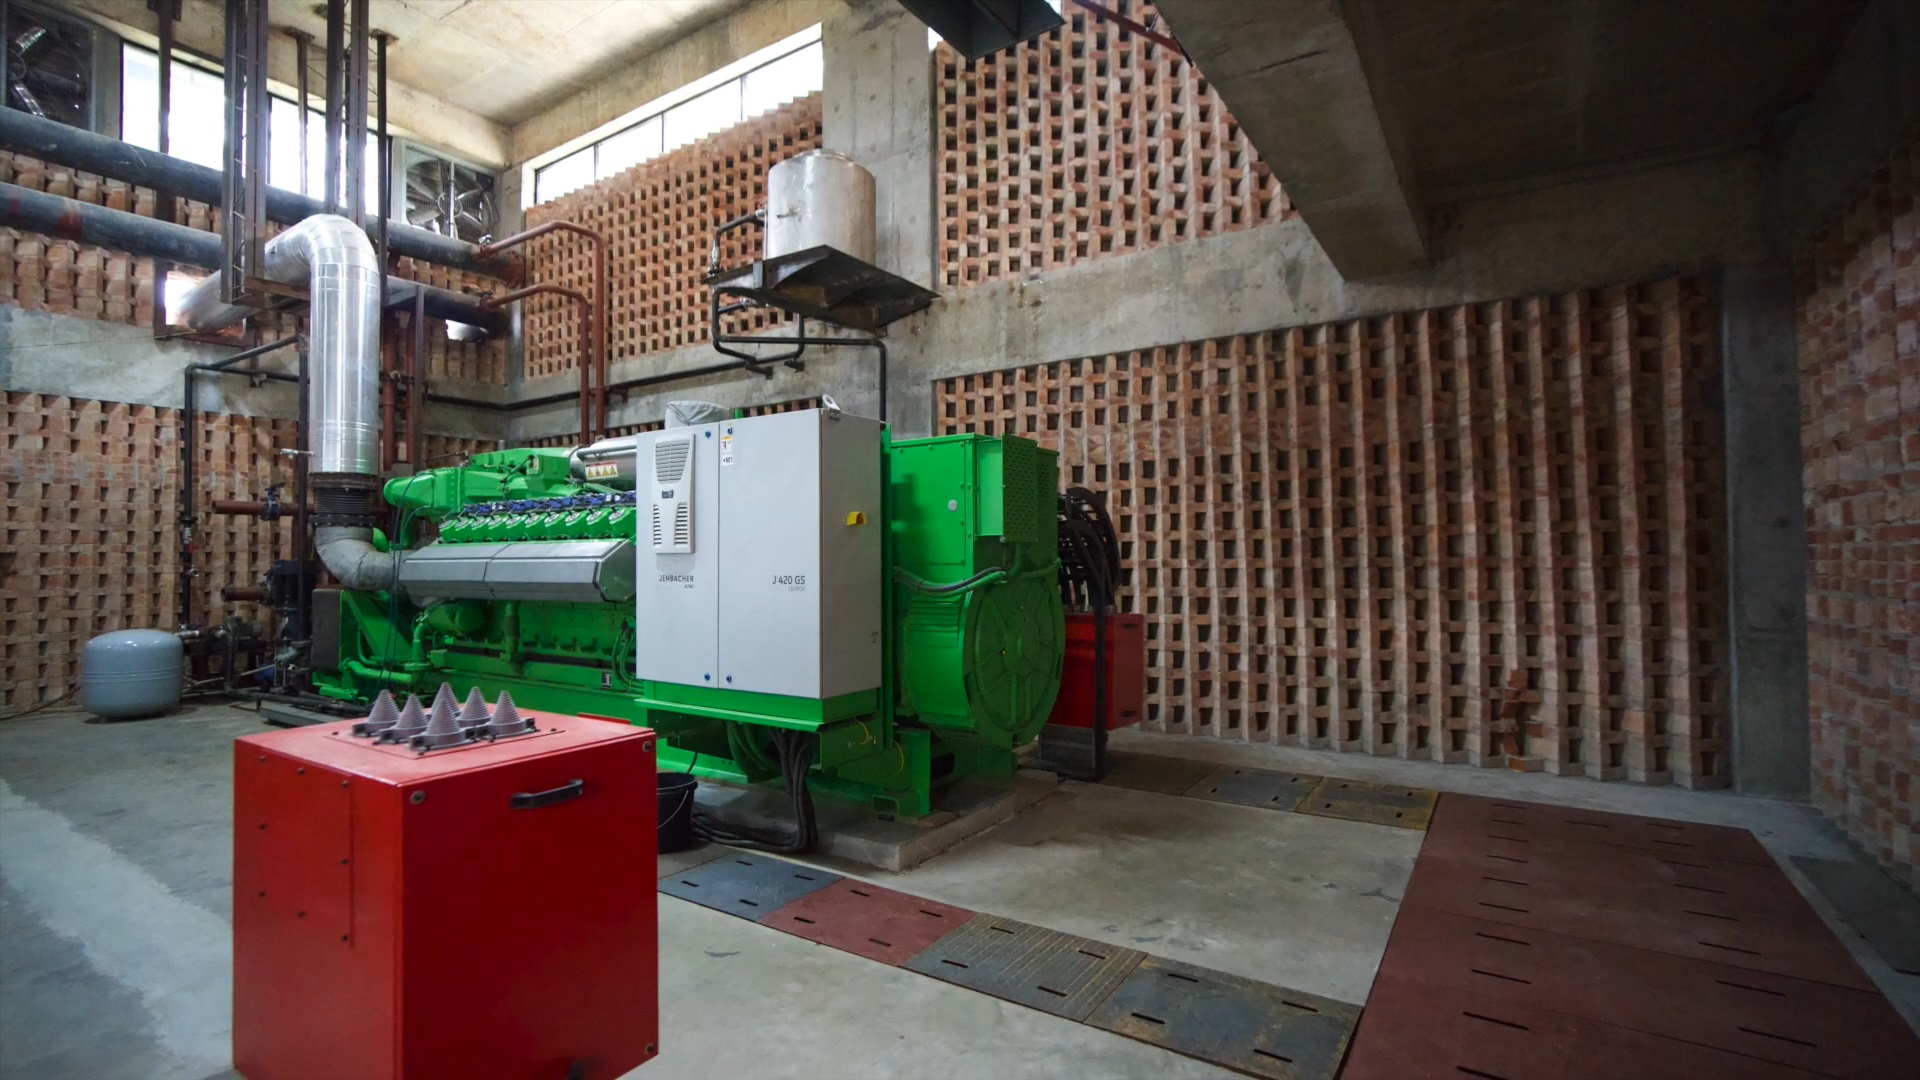
\includegraphics[width=1\linewidth]{figs/generator.jpg}
    \caption{Generator machine}
    \label{fig:generator}
\end{figure}

Generators play a crucial role in the textile industry by providing a reliable uninterrupted source of power.  
At the textile manufacturing facility, the significance of reliable power sources in maintaining seamless operations was observed.
\begin{figure}
    \centering
    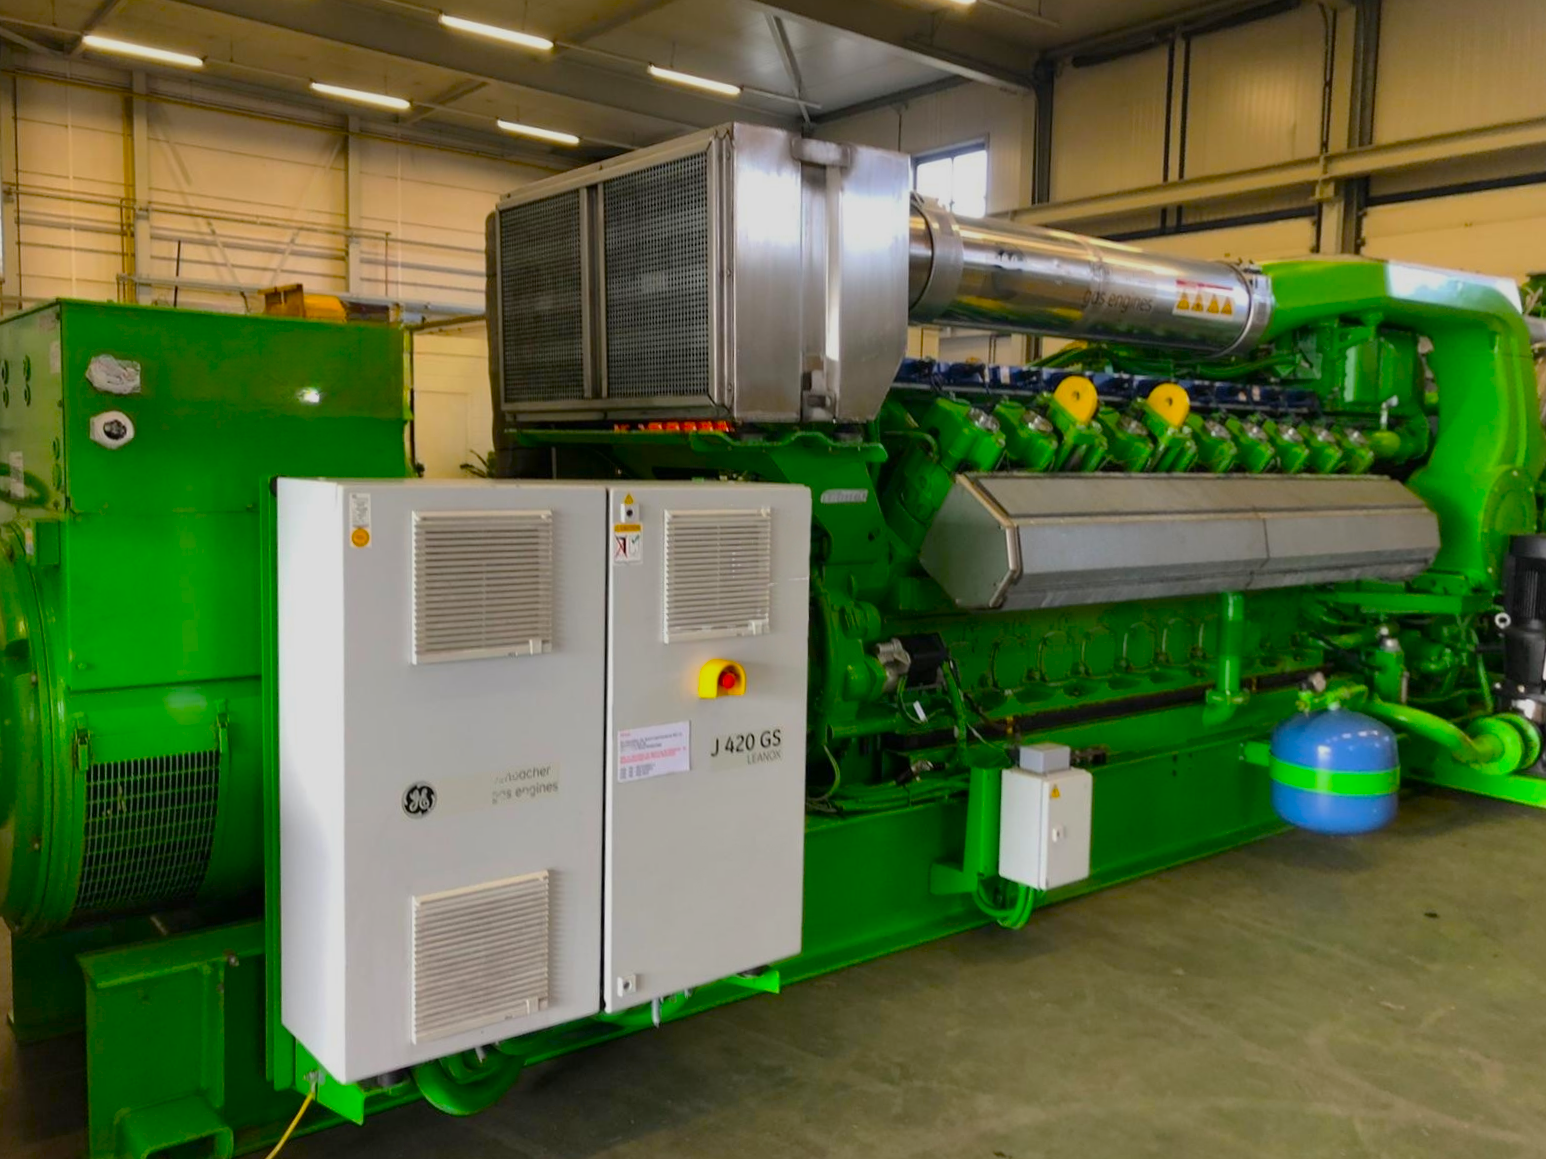
\includegraphics[width=1\linewidth]{figs/gas_gen_j420_leandx.png}
    \caption{Gas powered generator J420 LEANDX}
    \label{fig:gas_gen}
\end{figure}

The generator machine shown in Figure \ref{fig:generator} is the gas-powered generator J420 LEANDX, installed on the second floor of the energy building.

The generator offers an electrical output between 1,411 kW and 1,562 kW and a thermal output of 1,422 kW to 1,906 kW. Operating within a voltage range of 480V to 13.8kV, it achieves an electrical efficiency of up to 44.0\% and a thermal efficiency of up to 50.5\%. Such specifications make it well-suited to meet the high energy demands of the facility.
